\documentclass{article}
\usepackage[parfill]{parskip}
\usepackage[utf8]{inputenc}
\usepackage{amsmath}
\usepackage{amsthm} % for proofs
\usepackage{amssymb}
\usepackage{graphicx}
\usepackage{bm}
\usepackage[toc,page]{appendix}
\graphicspath{ {./images} }

\newcommand\norm[1]{\left\lVert#1\right\rVert}

\title{Covariance}
\author{Dávid Iván}

\begin{document}

\maketitle

\tableofcontents

\newpage



\section{Cholesky decomposition of the covariance}

Since the covariance matrix $P \in \mathbb{R}^{n\times n}$ is symmetric positive-definite, we can apply the Cholesky decomposition:

\begin{equation}\label{eq:Cholesky}
    P = L L^T
\end{equation}

where $L \in \mathbb{R}^{n\times n}$ is a lower triangular matrix. Let's apply SVD to it.

\begin{equation}
    L = U S V^T = \sum_{i=1}^{n} \sigma_i u_i v_i^T
\end{equation}

$\sigma_i > 0$ ($i=1, 2, \dots n$) are the singular values of $L$, $u_i \in \mathbb{R}^n$ ($i=1, 2, \dots n$) are the left singular vectors, and $v_i \in \mathbb{R}^n$ ($i=1, 2, \dots n$) are the right singular vectors of $L$. 

With this we can express both $L^T$ and $L^{-1}$:

\begin{equation}
    L^T = V S^T U^T = V S U^T = \sum_{i=1}^{n} \sigma_i v_i u_i^T
\end{equation}

\begin{equation}\label{eq:Linv}
    L^{-1} = V S^{-1} U^T = \sum_{i=1}^{n} \frac{1}{\sigma_i} v_i u_i^T
\end{equation}

Let's express P:

\begin{equation}
    P = LL^T = (USV^T) (VSU^T) = US^2U^T = \sum_{i=1}^{n} \sigma_i^2 u_i u_i^T
\end{equation}

This is the eigendecomposition of $P$, so its eigenvalues are $\sigma_i^2$, its eigenvectors are $u_i$.

\subsection{Numerical example}

Consider the folloing covariance matrix:

\begin{equation}
    P = \begin{bmatrix}
    2 & 0.5 \\
    0.5 & 1 \\
    \end{bmatrix}
\end{equation}

The Cholesky decomposition is:

\begin{equation}
    P = L L^T
\end{equation}

where

\begin{equation}
    L = \begin{bmatrix}
    1.4142 & 0 \\
    0.3536 & 0.9354 \\
    \end{bmatrix}
\end{equation}

The SVD of $L$:

\begin{equation}
\begin{split}
    L &= \sigma_1 u_1 v_1^T + \sigma_2 u_2 v_2^T \\
    &= 1.4856 \cdot \begin{bmatrix} -0.9239 \\ -0.3827 \end{bmatrix} \cdot \begin{bmatrix} -0.9705 & -0.2410 \end{bmatrix} \\
    &+ 0.8904 \cdot \begin{bmatrix} -0.3827 \\ 0.9239 \end{bmatrix} \cdot \begin{bmatrix} -0.2410 & 0.9705 \end{bmatrix}
\end{split}
\end{equation}

\begin{figure}[ht]
 \centering
  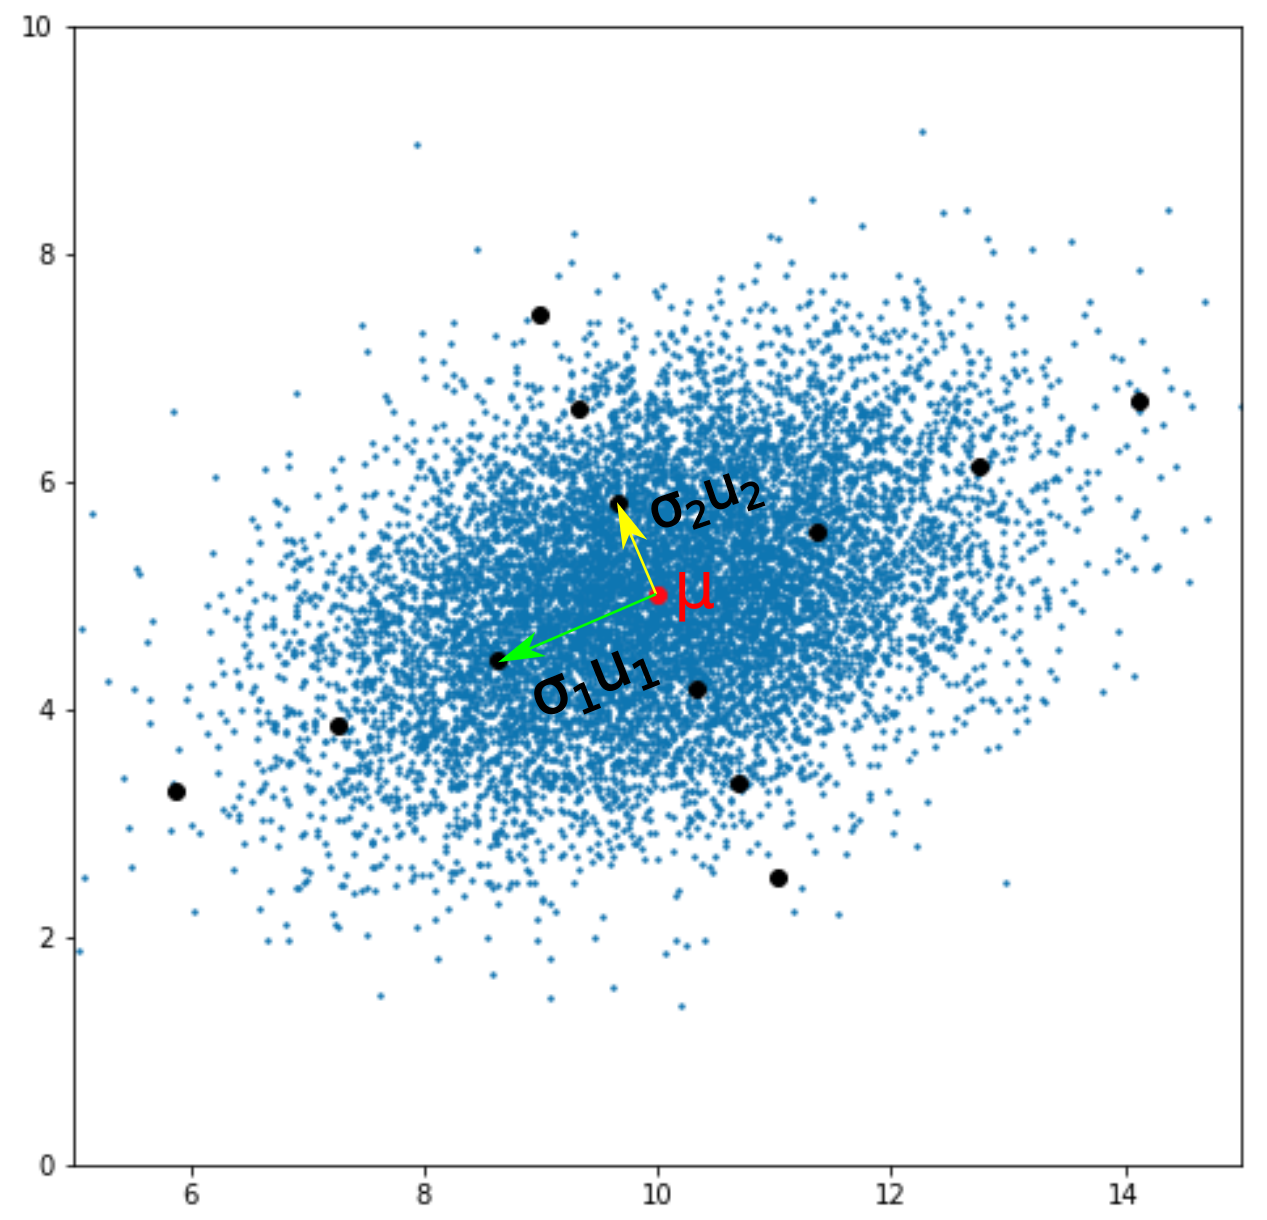
\includegraphics[width=230pt]{images/SVD_annot.png}
 \caption{Illustration of the eigenvectors and singular values.}
\end{figure}

\section{Standardization}

How to standardize a multivariate normal distribution? $X \sim N(\mu, P) \in \mathbb{R}^n$ is normally distributed with mean $\mu$, covariance $P$.

\begin{equation}\label{eq:standard}
    \boxed{Z = L^{-1} (X - \mu)}
\end{equation}

Where $L$ comes from equation (\ref{eq:Cholesky}). It is clear that $Z$ is normally distributed, since it is a linear transformation of the normal $X$. The mean:

\begin{equation}
    E(Z) = L^{-1} (E(X) - \mu) = L^{-1} (\mu - \mu) = 0
\end{equation}

The covariance:

\begin{equation}
\begin{split}
    P_Z &= Var(Z) = Var(L^{-1} (X - \mu))\\
    &= Var(L^{-1} X) = L^{-1} Var(X) L^{-T}\\
    &= L^{-1} LL^T L^{-T} = I
\end{split}
\end{equation}

So we see that $Z \sim N(0, I)$, i.e., it is standard normally distributed.

\section{Mahalanobis distance and Chi square}

The Mahalanobis (squared) distance is defined as

\begin{equation}
    d^2_M(x; \mu, P) = (x-\mu)^T P^{-1} (x-\mu)
\end{equation}

where $\mu, x \in \mathbb{R}^n$, $P \in \mathbb{R}^{n\times n}$ is a symmetric positive-definite matrix (the covariance).

Assuming that $X$ is normally distributed with $\mu$ mean, and $P$ (nonsingular) covariance, how is $d^2(X; \mu, P)$ distributed?

We know that $Z^TZ\sim \chi_n^2$, where $Z$ comes from the standardization of $X$, equation (\ref{eq:standard}).

\begin{equation}
    \begin{split}
        Z^T Z &= (X-\mu)^T L^{-T} L^{-1} (X-\mu) \\
        &= (X-\mu)^T (LL^T)^{-1} (X-\mu) \\
        &= (X-\mu)^T P^{-1} (X-\mu) \\
        &= d_M^2(X; \mu, P) \\
        & \sim \chi_n^2
    \end{split}
\end{equation}

So the Mahalanobis squared distance $d_M^2(X; \mu, P)$ is Chi-squared distributed with $n$ degrees of freedom.


\section{How to visualize Covariance}



\subsection{Points $c^2$ from the mean}

How to find those points that are in a specific Mahalanobis distance from the mean ($\mu$)? 

Construct the following vector ($\alpha_1, \alpha_2 \in \mathbb{R}$):

\begin{equation}
    x = \mu + \sum_{i=1}^{n}\alpha_i \sigma_i u_i
\end{equation}

The Mahalanobis squared distance is:

\begin{equation}
    \begin{split}
        d_M^2(x; \mu, P) &= (x - \mu)^T P^{-1} (x-\mu) \\
        &= (x - \mu)^T L^{-T} L^{-1} (x - \mu) \\
        &= \norm{ L^{-1} (x - \mu) }^2 \\
        &= \norm{ \sum_{i=1}^{n} \alpha_i \sigma_i L^{-1} u_i }^2 \\
        &= \norm{ \sum_{i=1}^{n} \alpha_i \sigma_i \frac{1}{\sigma_i} v_i }^2 \\
        &= \norm{ \sum_{i=1}^{n} \alpha_i v_i }^2 \\
        &= \sum_{i=1}^{n} \alpha_i^2
    \end{split}
\end{equation}

We used equation (\ref{eq:Linv}) to compute $L^{-1}u_i$. So if we seek vectors $x$ for which the Mahalanobis squared distance is $c^2$, then we can construct it by picking a point on the n-dimensional sphere with radius $c$, i.e.,

\begin{equation}
    \sum_{i=1}^{n} \alpha_i^2 = c^2
\end{equation}

Once we have a specific $\alpha$, we can construct $x$. For this $x(\alpha)$, $d_M^2(x(\alpha); \mu, P)=c^2$

\subsection{How to find $c^2$?}

Say I want to find a $c^2$ for which it is $95\%$ probable that $d_M^2(X; \mu, P) < c^2$, where $X \sim N(\mu, P)$. This is easy, since we know that $d_M^2(X; \mu, P) \sim \chi_n^2$. We need the quantile function (or percent point function) of the Chi-squared distribution.

\begin{equation}
    c^2 = Q_{\chi_n^2} (0.95)
\end{equation}

In 2 dimensions, $Q_{\chi_n^2} (0.95) = 5.99$.

\subsection{Example}

In 2 dimensions, we have $\alpha_1$ and $\alpha_2$. With $t \in (0, 2\pi)$

\begin{equation}
    \alpha_1 = c \cdot \sin(t)
\end{equation}

\begin{equation}
    \alpha_2 = c \cdot \cos(t)
\end{equation}

The following figure shows the ellipse for this scenario.

\begin{figure}[ht]
 \centering
  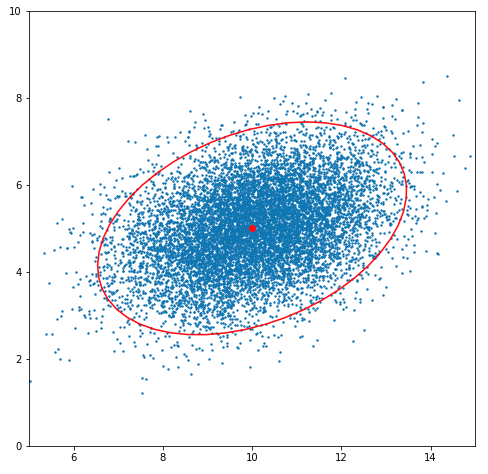
\includegraphics[width=230pt]{images/cov_example.png}
 \caption{ellipse of the 95\% confidence region.}
\end{figure}

\end{document}